\documentclass[12pt,twoside, a4paper, twocolumn]{article}
\usepackage[utf8]{inputenc}
\usepackage[brazil]{babel}
\usepackage[margin = 0.5in]{geometry}
\usepackage{amsmath}
\usepackage{amsthm}
\usepackage{amssymb}
\usepackage{amsthm}
\usepackage{setspace}
\usepackage[americanvoltages,fulldiodes,siunitx]{circuitikz}
\usepackage{lipsum}
\usepackage{pgfplots}
\usepackage{ifthen}
\usepackage{adjustbox}
\usepackage[section]{placeins}
\usepackage{hyperref}
\usepackage{graphicx}
\usepackage{amsmath}
\usepackage{amsthm}
\usepackage{amssymb}
\usepackage{amsthm}
\usepackage{setspace}
\usepackage[americanvoltages,fulldiodes,siunitx]{circuitikz}
\usepackage{lipsum}
\usepackage{pgfplots}
\usepackage{ifthen}
\usepackage{adjustbox}
\usepackage[section]{placeins}
\usepackage{hyperref}
\usepackage{graphicx}
\usepackage{adjustbox}
\pgfplotsset{compat=newest}
\graphicspath{ {./images/} }
%  #1 color - optional #2 x_0 #3 y_0 #4 x_f #5 y_f #6 name - optional  #7 true if adding lines to axis
\newcommand{\drawvector} [9] [color=cyan] {
 \draw[line width=1.5pt,#1,-stealth](axis cs: #2, #3)--(axis cs: #4, #5) node[anchor=south west]{$#6$};
\ifthenelse{\equal{#7}{true}}{
 \draw[line width=1pt,#1, dashed](axis cs: #4, #5)--(axis cs: #4, 0) node[anchor= north west]{$#8$};
 \draw[line width=1pt,#1, dashed](axis cs: #4, #5)--(axis cs: 0, #5) node[anchor=south east]{$#9$};
 }
 {}
}
\newcommand\deriv[2]{\frac{\mathrm d #1}{\mathrm d #2}}
\title{Sexto Relatório de Lab de Circuitos}
\author{Henrique da Silva \\ hpsilva@proton.me}
\date{\today}
\pgfplotsset{width = 10cm, compat = 1.9}
\begin{document}
\maketitle
\pagenumbering{gobble}
\newpage
%pagenumbering{roman}
\tableofcontents
\newpage



\section{Introdução}

\subparagraph*{Neste relatório vamos discutir um circuito com um AmpOp e dois capacitores que se comportara como um circuito RLC.}

\subparagraph*{Todos arquivos utilizados para criar este relatório, é o relatorio em si estão em:  \url{https://github.com/Shapis/ufpe_ee/tree/main/4th semester/lab circuitos}}


\section{Analise do circuito}

\begin{adjustbox}{scale=0.6}
    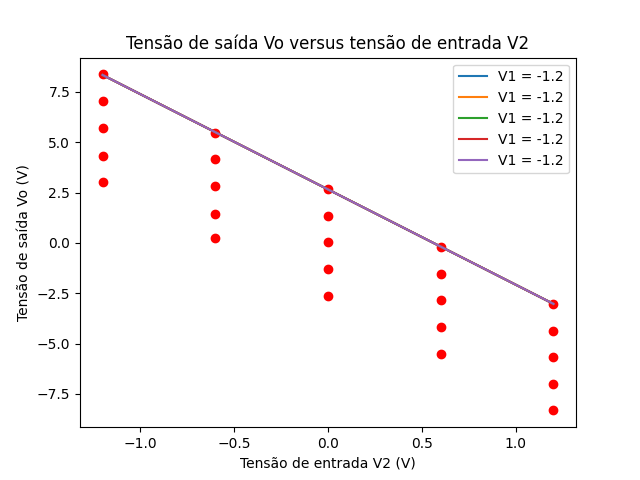
\includegraphics{Figure_2.png}
\end{adjustbox}

\subparagraph*{Fazendo análise nodal no circuito chegamos as seguintes equações:)

\begin{equation}
    \begin{aligned}
         & \frac{V_a - V_i}{R_1} + \frac{V_a - V_0}{R_2} + \frac{V_a}{R_3} + C_1 \deriv{V_a}{t} = 0 \\
         & \frac{-V_a}{R_3} - C_2 \deriv{V_0}{t} = 0                                                \\
    \end{aligned}
\end{equation}

\subparagraph*{Dai segue que:}

\begin{equation}
    \begin{aligned}
         & V_a = - R_3 C_2 \deriv{V_0}{t}                                                                                          \\
         & V_a \left(\frac{1}{R_1} + \frac{1}{R_2} + \frac{1}{R_3}\right) + C_1 \deriv{V_a}{t} - \frac{V_0}{R_2} = \frac{V_i}{R_1} \\
         & K = \left(\frac{1}{R_1} + \frac{1}{R_2} + \frac{1}{R_3}\right)                                                          \\
         & K V_a  + C_1 \deriv{V_a}{t} - \frac{V_0}{R_2} =\frac{V_i}{R_1}                                                          \\
    \end{aligned}
\end{equation}

\subparagraph*{Substituindo $V_a$ temos:}

\begin{equation}
    \begin{aligned}
         & C_1 C_2 R_3 \frac{d^2 V_0}{dt} + R_3 C_2 K \deriv{V_0}{t}    + \frac{V_0}{R_2} = -\frac{V_i}{R_1}              \\
         & \frac{d^2 V_0}{dt} + \frac{K}{C1} \frac{V_0}{dt} + \frac{V_0}{R_2 C_1 C_2 R_3} = - \frac{V_i}{R_1 C_1 C_2 R_3} \\
         & \frac{d^2 V_0}{dt} + 662.86 \frac{V_0}{dt} + 4456327.98 V_0 = - 3128911.14 V_i                                 \\
    \end{aligned}
\end{equation}

\subparagraph*{E tiramos as seguintes condições iniciais do circuito:}

\begin{equation}
    \begin{aligned}
         & V_0(0)  = - V_{C20}                          \\
         & \frac{V_0}{dt}(0) = -\frac{V_{C10}}{R_3 C_2}
    \end{aligned}
\end{equation}

\section{Analisando um exemplo}

\paragraph*{Para analisar um exemplo vamos usar os seguintes valores:}

\begin{center}
    \begin{tabular}{ |ccc| }
        \hline
        $R_1$ & $\rightarrow$ & $47K\varOmega$ \\
        $R_2$ & $\rightarrow$ & $33K\varOmega$ \\
        $R_3$ & $\rightarrow$ & $68K\varOmega$ \\
        $C_1$ & $\rightarrow$ & $100nF$        \\
        $C_2$ & $\rightarrow$ & $1nF$          \\

        \hline
    \end{tabular}
\end{center}

\subparagraph*{Sabendo que a solucao eh da forma:}

\begin{equation*}
    s^2 + 2 \alpha s + w_0{^2} = 0
\end{equation*}

\subparagraph*{Podemos utilizar a equação (3) e chegar às seguintes conclusoes:}

\begin{equation}
    \begin{aligned}
         & \alpha = \frac{R_3 C_2 K }{2 C_1 C_2 R_3} = 331.43 \\
         & w_0 = \sqrt{ \frac{1}{R_2 C_1 C_2 R_3}}= 2111.00   \\
    \end{aligned}
\end{equation}

\subparagraph*{Que nos indica que estamos num sistema subamortecido já que $w_0 > \alpha$, e que tem como solução a seguinte equacao:}

\begin{equation}
    \begin{aligned}
         & V_0(t) = K_1 e^{-\alpha} \cos{w_d t} + K_2 e^{-\alpha} \sin{w_d t} \\
         & w_d = \sqrt{w_0^2 - \alpha^2} = 2087.90                            \\
    \end{aligned}
\end{equation}

\subparagraph*{E podemos resolver para a condição inicial e conseguir o seguinte sistema de equações:}

\begin{equation}
    \begin{aligned}
         & V_0(0) = -V_{C20} = K_1 e^{-\alpha}              \\
         & V_0'(0) = -V_{C10} = K_2 e^{-\alpha} w_d R_3 C_2
    \end{aligned}
\end{equation}

\subparagraph*{Resolvendo numericamente na calculadora obtive a seguinte solução:}

\subparagraph*{$((0.702 V_i - V_{C20})*\cos{(2084.82t)}+3.18*e^{-58}*(2.01*e^{58}*V_i-1.27*10^{60}*V_{C10}-2.867*10^{58}*V_{C20})*sin(2084.82t))*e^{(-331.43t)} - 0.7021 * V_i$}


\subparagraph*{Simplificando com Wolfram Alpha na seguinte url \url{shorturl.at/adnEU} obtenho a seguinte equacao:}

\begin{equation}
    V(t) = e^{-331.43t} - 0.7021 * V_i
\end{equation}

\subparagraph*{Estou na duvida se isso deveria ter sinal invertido, as equações ficam grandes e difícil de passar de um meio (calculadora) para outro (computador no Wolfram) para simplificar, eu chequei bastante e não achei erro, mas intuitivamente eu imaginaria que o sinal de $V_i$ deveria ser positivo.}

\section{Resultados que deveria ter levado para o Lab}

\subsection{Porcentagem de $V_i$ para $t \rightarrow \infty$}
\subparagraph*{Como vimos na equação (8), para t tendendo a infinito teremos $V(t) = -0.7021 Vi$, ou seja, a tensão em módulo será de 70.21\% da tensão de entrada.}

\subsection{Curva de resposta natural para 8 vezes inverso de alpha}

\begin{adjustbox}{scale=0.55}
    \includegraphics{Figure_3.png}
\end{adjustbox}


\subsection{Curva de resposta forçada para 8 vezes inverso de alpha}

\begin{adjustbox}{scale=0.55}
    \includegraphics{Figure_4.png}
\end{adjustbox}

\subsection{Tempos de subida da resposta forcada:}

\begin{equation*}
    \begin{align*}
         & T_{s10} = 0.00022s \\
         & T_{s90} = 0.00077s \\
    \end{align*}
\end{equation*}

\subsection{Tempo de descida da resposta natural:}

\begin{equation*}
    \begin{align*}
         & T_{d10} =  0.00022s  \\
         & T_{d90} = s  0.00077 \\
    \end{align*}
\end{equation*}

\subsection{Overshoot natural}

\begin{equation*}
    \begin{align*}
         & T = 0.0015s \\
         & V = 2.124V  \\
    \end{align*}
\end{equation*}

\subsection{Overshoot Forcado}

\begin{equation*}
    \begin{align*}
         & T = 0.0015s \\
         & V = -2.124V \\
    \end{align*}
\end{equation*}

\newpage

\clearpage

\section{Medições no laboratório}

\subsection{Valores reais das partes.}
\subparagraph*{Abaixo estão os valores medidos das partes utilizadas no experimento:}

\begin{center}
    \begin{tabular}{ |ccc| }
        \hline
        $R_1$ & $\rightarrow$ & $46.34K\varOmega$ \\
        $R_2$ & $\rightarrow$ & $32.21K\varOmega$ \\
        $R_3$ & $\rightarrow$ & $67.1K\varOmega$  \\
        $C_1$ & $\rightarrow$ & $1.05nF$          \\
        $C_2$ & $\rightarrow$ & $101.56nF$        \\

        \hline
    \end{tabular}
\end{center}

\subsection{Imagem da onda}

\begin{adjustbox}{scale=0.25}
    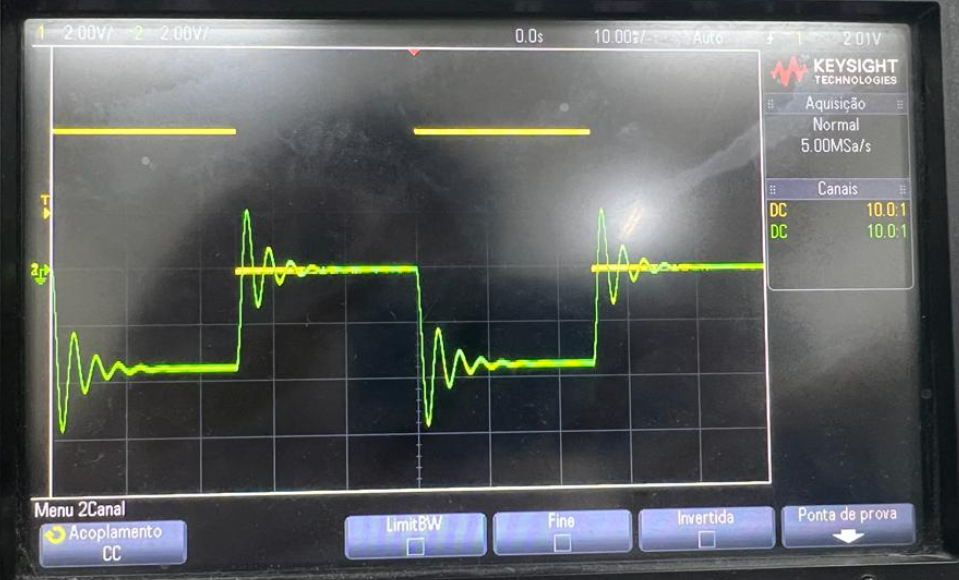
\includegraphics{Figure_1.png}
\end{adjustbox}

\subsection{Medições para o regime permanente}

\subparagraph*{Inicialmente medimos as tensões nos capacitores para tempos longos, ou seja. Quando estão em regime permanente, e obtivemos o seguinte:}

\begin{equation*}
    \begin{aligned}
        V_{C10} = -3.5V \\
        V_{C20} = 0V    \\
    \end{aligned}
\end{equation*}

\subsection{Resposta natural}

\subparagraph*{Obtivemos que em resposta natural, o capacitor $C_1$ em $t_0$ tem uma tensão de $-3.5V$, ele oscila de maneira subamortecida até tender a $0V$ em $t = \infty$.}

\subparagraph*{Já o mesmo capacitor $C_1$ em resposta forçada, inicia em $0V$ e oscila de maneira subamortecida até tender a $-3.5V$ em $t = \infty$.}

\subsection{Tempo de subida e descida}

\paragraph*{Utilizarei a frequência $f = \frac{1}{8} \alpha = 41.4$ para todos experimentos a seguir. Isto nos dará tempo suficiente para a tensão estabilizar.}

\begin{center}
    \begin{tabular}{ |ccc| }
        \hline
        $\%V$      & $t_{subida}$ & $t_{descida}$ \\
        $t_{10\%}$ & $200\mu s$   & $720 \mu s$   \\
        $t_{90\%}$ & $200\mu s$   & $900 \mu s$   \\
        \hline
    \end{tabular}
\end{center}

\subsection{Overshoot}

\begin{center}
    \begin{tabular}{ |ccc| }
        \hline
        $\,$             & $Tempo$  e $Tensão$              \\
        $T_{overshootN}$ & $1.45ms$            & $2.15V$    \\
        $T_{overshootF}$ & $1.4ms$             & $-2.0625V$ \\
        \hline
    \end{tabular}
\end{center}

\section{Conclusoes}

\subparagraph*{Os resultados obtidos em laboratório foram coerentes com os resultados teóricos. Algo que não bateu exatamente como eu esperava foi a medição da proporção entre a tensão no tempo infinito e a tensão de entrada. O módulo deste valor estava coerente, mas eu sinto que o sinal ficou invertido do que deveria ser.}

\end{document}